\section{The Red Giant Branch Bump in NGC 2808}
NGC 2808 is made up of of anywhere from 2 - 5 separate stellar populations. In
Chapter \ref{chap:ngc2808} we discussed modeling efforts of the primordial
and the most enriched of these populations (A and E). Here we identify the
RGBB location in both populations and compare that to observations of the RGBB
luminosity.

Identification of the RGBB may be performed with either isochrones or stellar
evolutionary tracks. For the same reasons laid out in \citet{Joyce2016} we use
evolutionary tracks in place of isochrones. This is primarily due to the
limited sampling of equivalent evolutionary points near the bump which can
result in the bump be interpolated over. 

We select two evolutionary tracks from the Population A (Y $\sim$ 0.24) and
Population E (Y $\sim$ 0.36) model sets each of a mass so that they reach the
red giant branch within 100 Myr of each other. The population A model is of
mass 0.857 M$_{\odot}$ while the population E model is of mass 0.625
M$_{\odot}$. Identification of the RGBB in the tracks is then straightforward.
First we perform bolometric corrections to take the tracks into WFC3/ACS
filters with the same distance modulus and extinction as we fit in Chapter
\ref{chap:ngc2808}, then we identify the maximum of the derivative of F814W
magnitude vs. age. This metric proves to reliably extract the center of the
RGBB. We identify the bump in population A at an F814W magnitude of approximately 16.5 while
we are unable to identify the gap in population E.

In order to verify this is a attribute of the population and not the particular
model we selected we perform stellar population synthesis using the best fit
isochrones from Chapter \ref{chap:ngc2808}. This is done using the population
synthesis module in \fidanka. Further, HUGS artificial star tests are used in
order to inject proper uncertainties and to model completeness. Figure
\ref{fig:LumFAE} shows both the synthetic population (left) and the luminosity
function of that population (right). We measure the magnitude of the RGBB by
first flattening the luminosity function shown in Figure \ref{fig:LumFAE} with
a second order polynomial. We then fit a Gaussian model --- with a prior of
16.5 as the mean of the RGBB magnitude --- to the flattened luminosity function.
We find that the RGBB in population A is located at F814W = 16.53$\pm$0.004
mag, this is in agreement with literature values for the magnitude of the RGBB
in NGC 2808. However, once again we do not see a bump in the synthetic
population E data. The pertinent question then becomes why do we not see a
RGBB in population E when compared to population A.

\begin{figure}
  \centering
  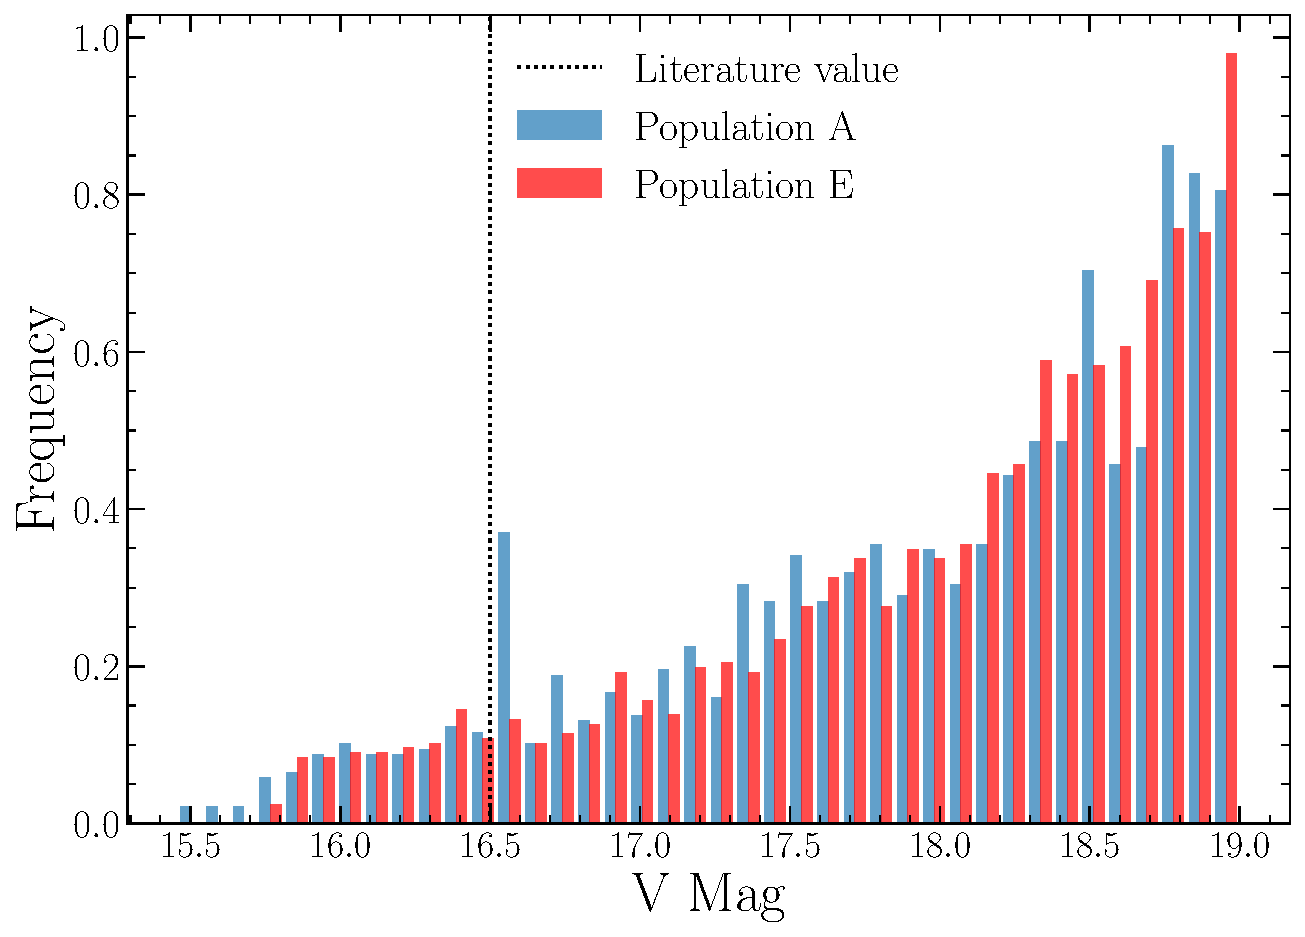
\includegraphics[width=0.85\textwidth]{figures/rgbb/ComparisonOfRGBBump.pdf}
  \caption{Luminosity function for a population A and E model. Note how there
  is a bump at approximately $M_{V} = 16.5$ for population A but not for E. The
  dashed line represents the literature value for the observed RGBB in NGC
  2808.}
  \label{fig:LumFAE}
\end{figure}

\subsection{Population E and the Case of the Missing Bump}
It is well established that stars with lower metallicities will have a less
pronounced bump \citep{Cassisi2002, Bjork2006}. Due to Population E's
signifigantly enhances helium abundance the mean molecular mass ($\mu$) within
population E stars is approximatly 25\% larger than $\mu$ is for population A
stars. Higher mean mollecular masses steepen the adiabatic temperaure gradient
thus changing the depth at which a model is unstable to convection. Moreover,
the metallicity of population E is lower than that of population A. Lower
metallicities decrease the opacity of a star and therefore make the coupling
between the radiation field and the fluid field weaker. This results in less
efficient thermal transfer into the fluid of the star. Consequently, models have
a more shallow outer convective zone (Figures \ref{fig:convEnvMass} \&
\ref{fig:MfracVX}) which may not be able mix new hydrogen fuel both deep enough
within a model and early enough in a model's life to induce the RGBB.
Specifically, in population E we see that the convection zone only reaches down
50\% of the mass of the model (Figure \ref{fig:MfracVX}). Because of this,
shell burning does not reach the discontinuity in hydrogen mass fraction until
later in the model's life. Because the luminosity of the models is rapidly
increasing during this phase of evolution the timescales to burn hydrogen
shrink rapidly as well. Therefore, in population E even though there does seem
to be a small discontinuity in the hydrogen mass fraction, evolutionary time
scales are so short that the population will evolve through this period without
a noticeable bump. The lack of an observed RGB bump in Population E models ---
and the commensurate lack of effect that population E has on the location of
the NGC 2808 bump --- validates previous theoretical investigations of the bump
which have ignored the presence of multiple populations in NGC 2808 while
modeling the bump.

\begin{figure}
  \centering
  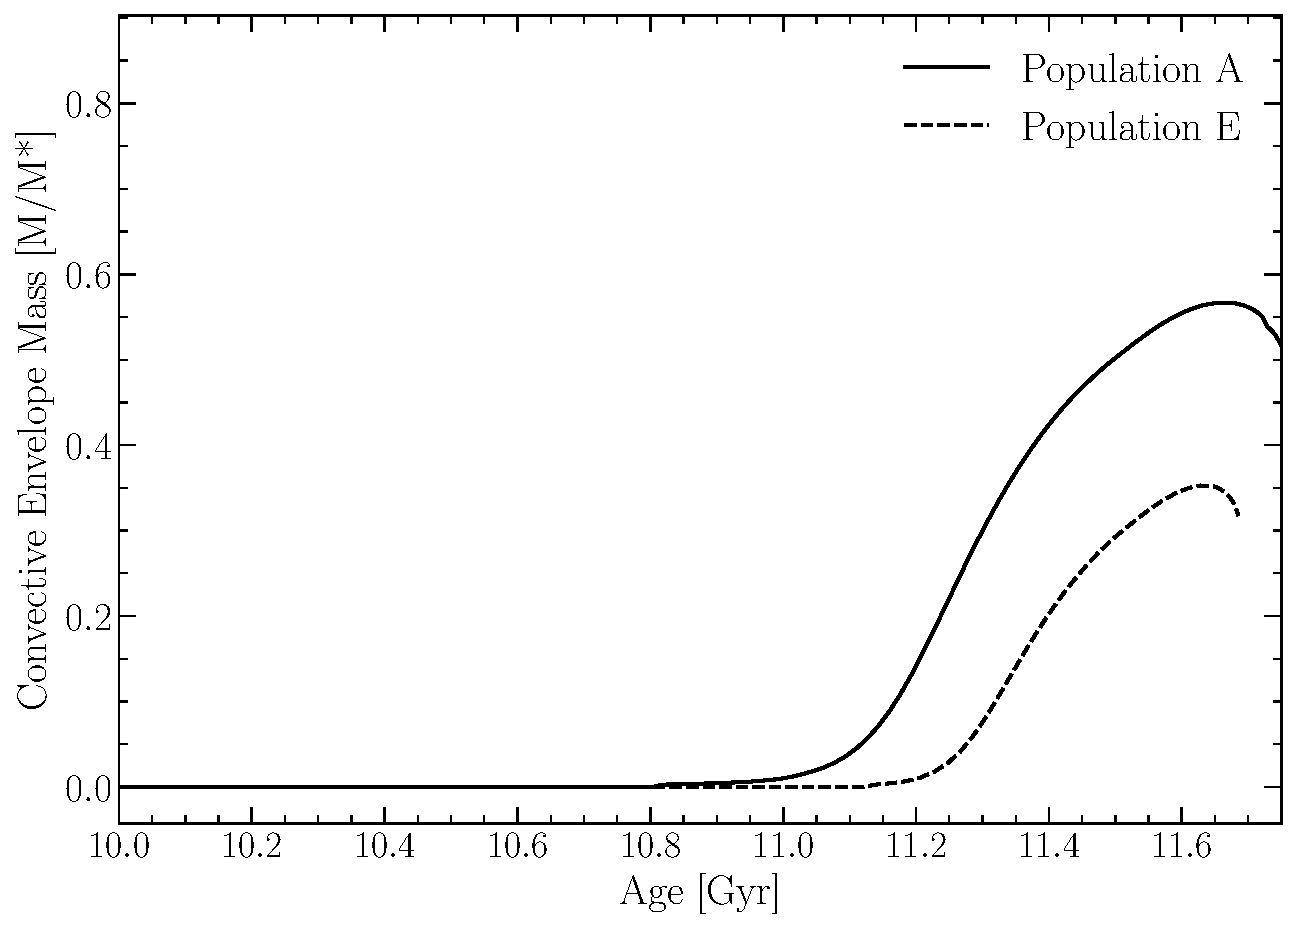
\includegraphics[width=0.85\textwidth]{figures/rgbb/ConvectiveEnvelopeMass.pdf}
  \caption{Fractional mass of the convective envelope of a population A and E
  model vs. model age. Note how the population A model's convective envelope
  reaches approximately 60 percent of the star by mass while the population E
  convective envelope only reaches 40 percent of the star by mass.}
  \label{fig:convEnvMass}
\end{figure}

\begin{figure}
    \centering
    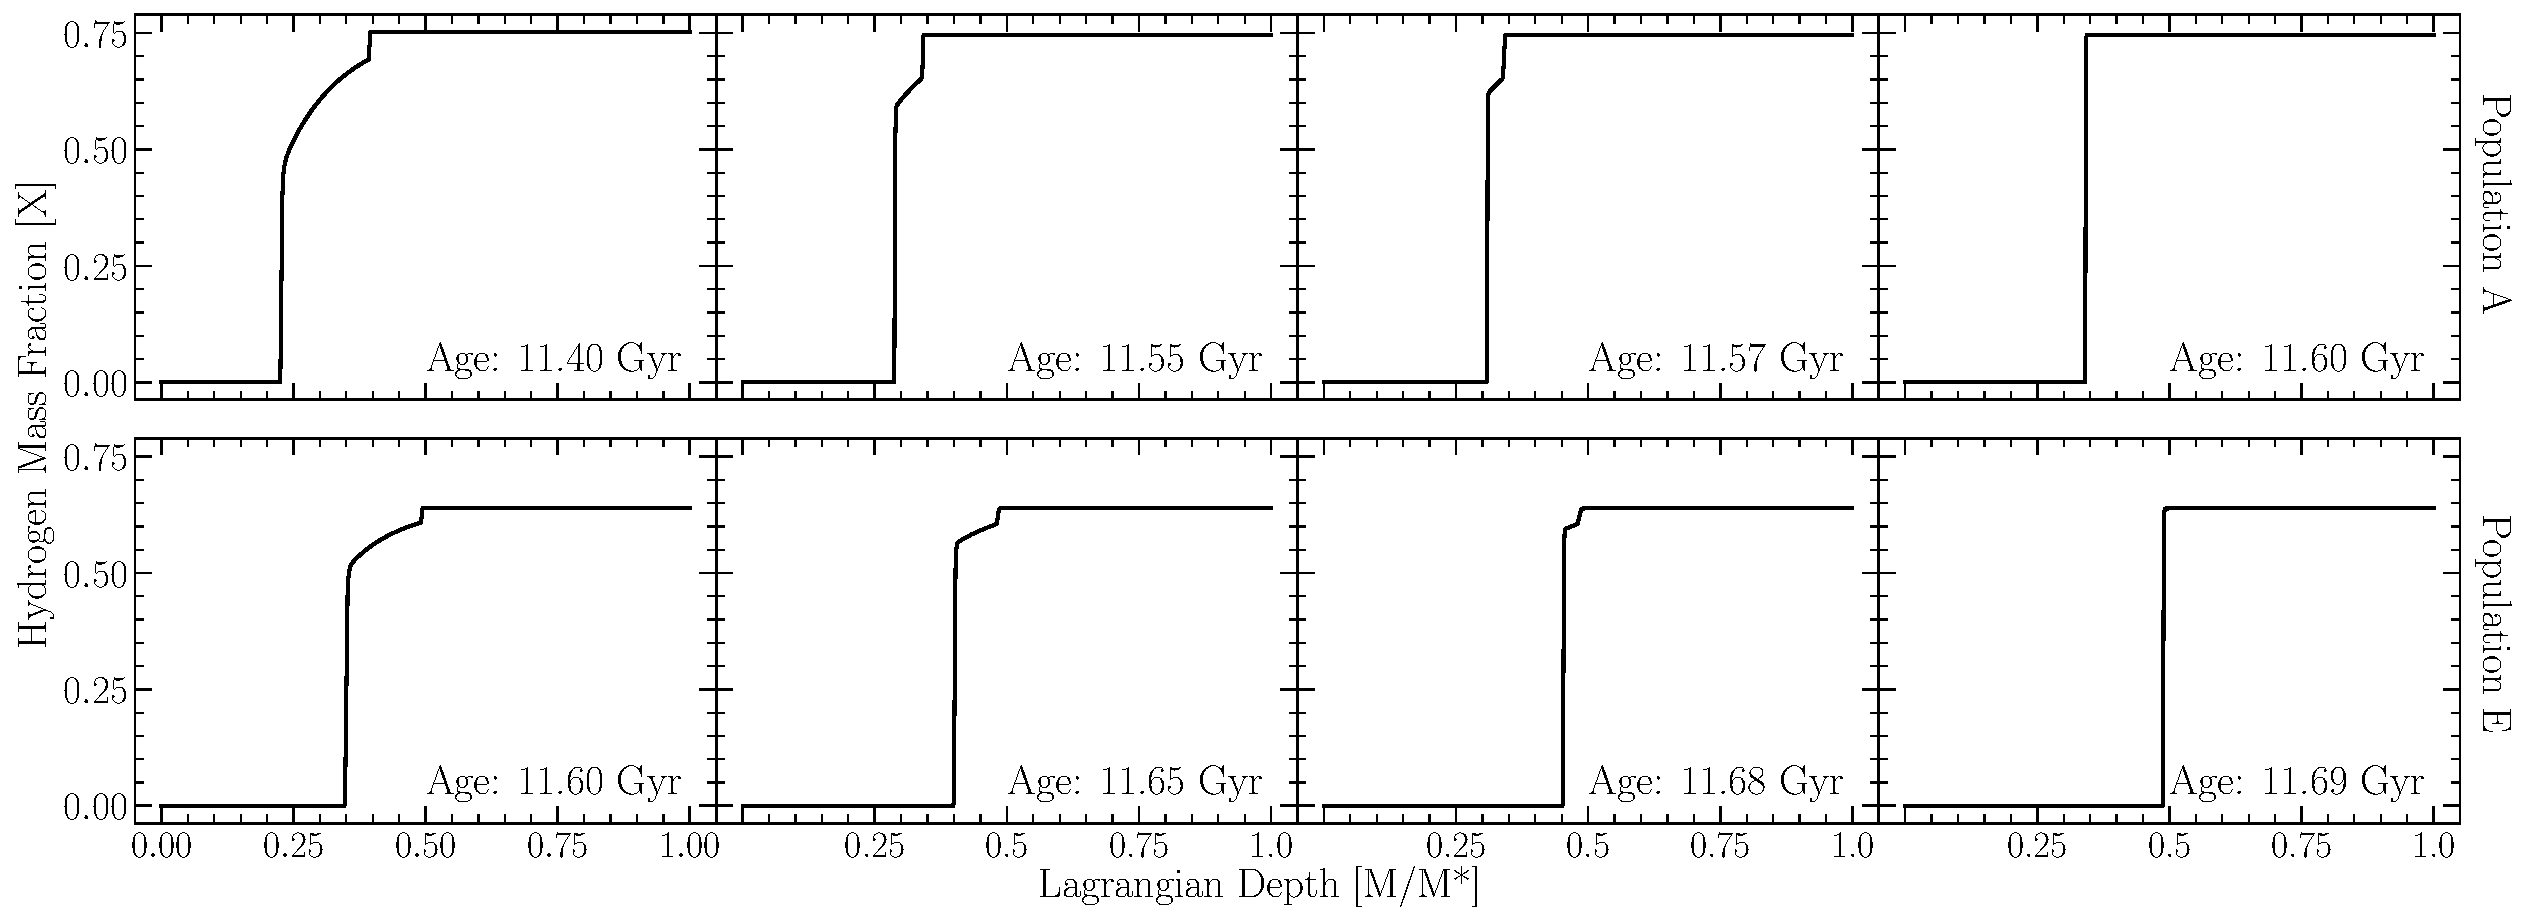
\includegraphics[width=\textwidth]{figures/rgbb/EvolutionAE.pdf}
    \caption{Evolution of the hydrogen mass fraction vs. the Lagrangian depth
    within Population A (top) and E (bottom) Stellar models. From left to right
    panels show snapshots at informative ages. Note how Population E does not
    exhibit the same deep bump in its hydrogen mass fraction as Population A
    does. Populations have been roughly mas calibrated so they reach the same
    evolutionary stages within 100 Myr of each other.}
    \label{fig:MfracVX}
\end{figure}
